\documentclass[11pt,a4paper,twocolumn,final]{article}
\usepackage[left=2.5cm,right=2.5cm,top=2.5cm,bottom=2.5cm]{geometry}
\usepackage[utf8]{inputenc}
\usepackage[portuguese]{babel}
\usepackage[T1]{fontenc}
\usepackage{amsmath}
\usepackage{amsfonts}
\usepackage{amssymb}
\usepackage{enumerate}
\usepackage{graphicx}
\usepackage{booktabs}
\usepackage{lipsum}
\usepackage{multirow}
\usepackage[hyphens]{url}
\usepackage{subfig}
\usepackage[T1]{fontenc}
\usepackage{fourier}
\usepackage{microtype}
\usepackage{csquotes}
\usepackage{siunitx}\sisetup{locale = FR}\DeclareMathSymbol{\comma}{\mathord}{letters}{"3B}
\columnsep = 1.0pc
\parindent = 0.0pt
\parskip = 6.0pt plus 2.0pt minus 2.0pt


%% TÍTULO
\title{\textsc{Estudo de Oscilações de Estados em Autômatos Celulares com Inércia}}
\author{ \textsc{Apresentado como Relatório Parcial de Iniciação Científica} \\\\Ly Sandro Amorim de Campos Salles \\
Departamento de Física – Universidade Federal do Paraná \\
Centro Politécnico – Jd. das Américas – 81531-990 – Curitiba – PR - Brasil \\
e-mail: lysandroacs@gmail.com\\\\Projeto realizado com Bolsa remunerada UFPR/TN do Edital PIBIC 2018/2019\\ Orientação pelo Prof. Dr. Marlus Koehler
}
\date{\today}


%% COMEÇO DO DOCUMENTO
\begin{document}

\twocolumn[
\maketitle
\begin{abstract}

	Utilizando o modelo de autômato celular proposto por Dietrich Stauffer em 2003 e a ideia de estudar aglomerados explorada por Klaus Kramer em 2014, foram estudados padrões recorrentes envolvendo o número de aglomerados e o estado médio em várias execuções do autômato celular desenvolvido durante o primeiro semestre de Iniciação Científica. Foi criado o termo \textit{afinidade} para autômatos celulares e descoberto que este independe da largura da matriz utilizada. Também foram explorados padrões de atratores e caos ao comparar o número de aglomerados com o valor médio de uma propriedade instrínseca a cada célula, chamada de limiar (ou inércia). Os próximos passos deste trabalho incluem a possível verificação da geração do potencial de Lennard-Jones através das simulações do autômato celular desenvolvido, o estudo de padrões de dinâmica não-linear e caos em alguns conjuntos de dados, e a exploração de autômatos celulares em dimensões maiores que 2.

\vspace{0.3cm}
%
\textbf{Palavras-chave}: autômatos celulares, autômatos com resistência, autômatos estocásticos, estudo de aglomerados.
%
\end{abstract}

\vspace{0.7cm}]

\section*{Pesquisa Bibliográfica}

Autômatos são objetos que operam a si mesmos. Essa definição, disponível na Encyclopaedia Britannica (Referências \cite{britannica1} e \cite{britannica2}), traz a possibilidade de objetos de uso cotidiano, como o computador e o celular, se encaixarem na categoria de autômatos. Porém, a existência de desses objetos não é nova, existindo autômatos desde a Grécia antiga na figura de um modelo de madeira de um pombo construído por Archytas de Tarentum. Utilizações contemporâneas de autômatos incluem as redes neurais e as inteligências artificiais. Também existem outros tipos famosos de autômatos, como os autômatos celulares.

Os autômatos celulares são, segundo a Encyclopaedia Britannica (referência \cite{britannica3}), simples modelos espacialmente distribuídos capazes de simular processos do mundo real. Eles foram inventados por John von Neumann e Stanislaw Ulam no Laboratório Nacional de Los Alamos em 1940 e ficaram famosos através do ``Game of Life'', inventado por John Conway em 1970, que simula a dinâmica de vida, morte e população.

Em 2003, Dietrich Stauffer (Referência \cite{stauffer}) publicou um artigo no qual ele descreveu um autômato celular não-homogêneo (chamado por ele de InCA ou Inhomogeneous Cellullar Automata) no qual a atualização das células ocorria de forma aleatória e cada célula tinha uma espécie de resistência interna a mudar de estado. Formalmente, em uma matriz, cada célula do autômato de Stauffer guarda dois números: o próprio estado e o próprio limiar. O limiar é definido como sendo o menor valor da soma dos estados das células vizinhas necessário para que a célula fique no estado $+1$ caso ela seja atualizada. Caso a célula seja atualizada mas ela não tenha um número de vizinhos no estado $+1$ suficiente para ficar no estado $+1$, a célula fica no estado $-1$ e seu limiar diminui por um número aleatório entre $0$ e $q$, onde $q$ é o ajuste máximo de limiar, definido antes do início da simulação. Caso a célula fique no estado $+1$ ao ser atualizada, o seu limiar aumenta por um número aleatório entre $0$ e $q$.

Em seu artigo ``Adjustment and social choice'' (Referência \cite{stauffer}), Stauffer explorou o comportamento das oscilações do estado médio e do limiar médio da matriz em função do tempo de simulação. Nisso ele percebeu que, quanto maior o valor do ajuste máximo de limiar $q$, maior é a frequência dessas oscilações em função do tempo. Stauffer utilizou os resultados obtidos para propor previsões e modelos para mercados financeiros.

Já em 2014, Klaus Kramer (Referência \cite{klaus}) desenvolveu estudos sobre autômatos celulares envolvendo três estados e focou na formação de aglomerados. Dos três estados, dois ($+1$ e $-1$) eram competitivamente ativos pois competiam entre si e um -- o estado $0$ -- era competitivamente passivo pois não competia com os outros estados. A regra de atualização utilizada foi semelhante à de Stauffer, com a diferença de o limiar de cada célula permanecer constante ao longo de toda a simulação. Além disso, nesse modelo as células com pelo menos uma célula vizinha no estado $0$ têm chances aleatórias de mudar para o estado $0$. Por fim, Kramer relacionou os estudos realizados com áreas de transição entre biomas diferentes.

Tendo como base esses autores, o objetivo deste trabalho foi explorar a dinâmica oscilatória do autômato celular de Stauffer, juntando a ele a ideia de estudar aglomerados empreendida por Kramer, a fim de buscar padrões que possam ser associados a fenômenos naturais.

\section*{Metodologia}

\subsection*{Estudos iniciais}

O primeiro passo para este estudo foi conhecer a produção científica sobre autômatos celulares na área da Física. Para isso foram lidos alguns artigos, incluindo:
\begin{enumerate}
    \item Rodrigo de Lazzari: “Estudo De Um Autômato Celular Para Modelar Ciclos De Expansão E Contração (“Boom E Burst”)” (Referência \cite{lazzari});
    \item Klaus Kramer: “Dinâmica de padrões em autômatos celulares com inércia” (Referência \cite{klaus});
    \item Gérard Weisbuch, Dietrich Stauffer: “Adjustment and social choice” (Referência \cite{stauffer});
\end{enumerate}
Também foram verificadas implementações de autômatos celulares  com o software de simulações científicas Netlogo. Ainda foi feita a leitura de alguns artigos sobre estatística e correlação para auxiliar na interpretação dos dados gerados pelas simulações. Adicionalmente, com o objetivo de obter conhecimento para criar implementações de autômatos celulares na linguagem de programação C, foram  lidos vários capítulos do livro “C programming: A modern approach, 2nd Edition” do autor K.N. King (Referência \cite{king}).
    
\subsection*{Desenvolvimentos}

O primeiro desenvolvimento foi a percepção de características recorrentes nos autômatos celulares observados nos Estudos Iniciais.
A seguinte lista de características de autômatos celulares foi produzida com base nos artigos e software explorados:\\
\underline{Número de estados:} Quantos estados cada célula pode assumir.\\
\underline{Competitividade ou simbiose entre estados:} se a existência de um estado favorece ou inibe, nas proximidades, a existência de estados diferentes.\\
\underline{Vizinhança interna:} a região que é considerada interna a cada célula.\\
\underline{Vizinhança externa:} a região que é considerada externa a cada célula, apesar de ser próxima o suficiente para afetar diretamente o comportamento da célula.\\
\underline{Determinismo ou estocasticidade:} se a atualização das células ocorre de maneira previsível ou aleatoriamente.\\
\underline{Topologia do espaço:} como as bordas ou células estão conectadas.\\
\underline{Geometria do espaço:} formato das células e organização delas no espaço, caso aplicável.\\
\underline{Regras para atualização das células:} regras que determinam qual será o estado da célula no próximo passo ou ciclo da simulação.\\
\underline{Superposição de estados:} se é possível que cada célula tenha mais de um estado ao mesmo tempo.\\
\underline{Propriedades intrínsecas a cada célula:} características únicas a cada célula, além do estado.

O autômatos celular não-homogêneo (InCA) de Stauffer foi modelado utilizando as características acima, resultando na descrição abaixo:\\
\underline{Número de estados:} Dois estados, -1 e 1.\\
\underline{Competitividade ou simbiose entre estados:} competitividade.\\
\underline{Topologia do espaço:} quadrada de tamanho $L\times L$, onde $L$ é a \textit{largura da matriz} em unidades de números de células, com bordas fechadas. Células conectadas verticalmente e horizontalmente por vizinhança mais próxima, mas não diagonalmente..\\
\underline{Geometria do espaço:} malha quadrada.\\
\underline{Vizinhança interna:} quadrada de raio 0 (somente a própria célula).\\
\underline{Vizinhança externa:} Cruz com eixos paralelos à malha da geometria do espaço. Raio 1. Formato de +. Vizinhança mais próxima. Células nas posições Norte, Sul, Leste e Oeste em relação à célula considerada.\\
\underline{Determinismo ou estocasticidade:} estocasticidade porque, em cada passo, uma célula escolhida aleatoriamente é atualizada com um parâmetro de valor aleatório.\\
\underline{Propriedades intrínsecas a cada célula:} cada célula $\mathbf{x}$ tem um valor intrínseco $\lambda_\mathbf{x}$, chamado \textit{limiar}, que determina qual a menor soma dos estados das células da vizinhança externa necessária para que a célula fique no estado +1 caso ela seja atualizada.\\
\underline{Regras para atualização das células:}  dada uma célula $\mathbf{x}$, caso ela seja atualizada, o limiar $\lambda_\mathbf{x}$ aumenta caso a célula fique +1 e diminui caso a célula fique -1. O valor $|\Delta\lambda_\mathbf{x}|$ é gerado aleatoriamente e está entre $0$ e $q$, onde $q$ é o \textit{ajuste máximo de limiar}.\\
\underline{Superposição de estados:} Não, somente um estado por célula.\\


Em seguida, esse modelo de autômatos celular foi implementado na linguagem C. Para cada simulação, a matriz foi inicializada com valores $-1$ ou $+1$ dispostos aleatoriamente mas de modo que a diferença entre o número de células positivas e o número de células negativas fosse menor que 1\% do número total de células na matriz. Para todas as células o limiar foi iniciado em $\lambda_\mathbf{x} = 0$. A Figura \ref{fig:matrizL100Ciclo0} exibe a matriz estado inicial gerada em uma execução do InCA implementado.

\begin{figure}
    \centering
    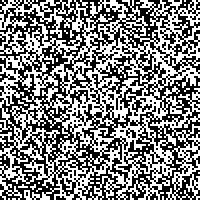
\includegraphics[width=0.7\linewidth]{matrizL100Ciclo0.png}
    \caption{Representação gráfica da matriz de estados iniciais de uma simulação com $L=100$. Células pretas representam o estado $-1$ e células brancas representam o estado $+1$. A matriz de estados iniciais é gerada de forma a manter o número de células positivas próximo ao número de células negativas.}
    \label{fig:matrizL100Ciclo0}
\end{figure}

O grande diferencial desta implementação do InCA, em relação ao estudo de Stauffer, foi a utilização de um algoritmo de contagem de aglomerados de células com o mesmo estado. Esse algoritmo, ilustrado na Figura \ref{fig:contamination}, encontra todas as células em um mesmo aglomerado através de ``contaminações'' sucessivas de células com o mesmo estado que são vizinhas entre si.

\begin{figure}
    \centering
    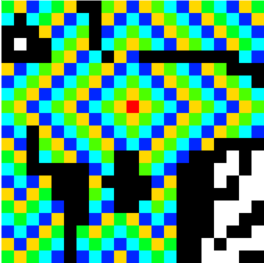
\includegraphics[width=.7\linewidth]{contamination.png}
    \caption{Algoritmo de contagem de aglomerados por contaminação de células vizinhas com o mesmo estado. Cada aglomerado é contaminado a partir de uma primeira célula até que não existam mais células a serem contaminadas. Na figura, a primeira célula é a central (em vermelho). Em seguida, as quatro células adjacentes a essa célula são contaminadas. No passo seguinte as oito células adjacentes a essas quatro células são contaminadas. O processo é repetido até que não existam mais células a serem contaminadas.}
    \label{fig:contamination}
\end{figure}

A implementação do InCA foi planejada para imprimir várias informações sobre a situação da matriz: Ciclo, Estado Médio da matriz, Limiar Médio da matriz, Número de Aglomerados e Índice de células Positivas que Pertencem a Algum Aglomerado (número total de células positivas em algum aglomerado dividido pelo número total de células na matriz). Um \textit{Ciclo} foi definido como sendo igual a $L\times L$ atualizações aleatórias de células na matriz, já que esse seria o número de atualizações de células caso o sistema fosse determinístico.

\subsection*{Metodologias de análise}

As análises foram feitas graficamente com os dados de estado médio, limiar médio, número de aglomerados e índice de células pertencentes a aglomerados em função do ciclo da simulação. Nesses gráficos foram buscados padrões recorrentes, como retas, parábolas ou elipses. Para isso foram feitas 288 simulações, variando a largura da matriz pelos valores 100, 250,
500,
750,
1000,
1250,
1500,
1750 e
2000, e o ajuste máximo de limiar entre os valores \num{0,5},
\num{0,75},
1,
\num{1,5},
2,
3,
4,
5,
6,
7,
8,
9,
10,
11,
12,
13,
14,
15,
16,
17,
18,
19,
20,
25,
30,
35,
40,
45,
50,
100,
150,
200 e
500.

\section*{Resultados Parciais Alcançados}

O primeiro estudo foi realizado quanto ao efeito da topologia no comportamento do valor médio e do limiar médio em função do ciclo. Foi observado que topologias com bordas conectadas apresentam gráficos mais suaves em relação a topologias com bordas fechadas. %Isso está ilustrado nas Figuras \ref{fig:topocaixa} e \ref{fig:topotorus}.

%\begin{figure}
%    \centering
%    \includegraphics[width=.9\linewidth]{topocaixa%.png}
%    \caption{Topologia de caixa}
%    \label{fig:topocaixa}
%\end{figure}
%
%\begin{figure}
%    \centering
%    \includegraphics[width=.9\linewidth]{topotorus%.png}
%    \caption{Topologia de Torus}
%    \label{fig:topotorus}
%\end{figure}

O segundo estudo foi feito quanto ao número de aglomerados e índice de células pertencentes a aglomerados. Também foi explorada a relação entre estado médio e número de aglomerados. Foi observado que o índice de células em aglomerados aumenta quando o estado médio fica positivo, como ilustrado na Figura \ref{fig:dataL2000Q100CellInClusterAvgStateVsCycle}. 
\begin{figure}[h]
    \centering
    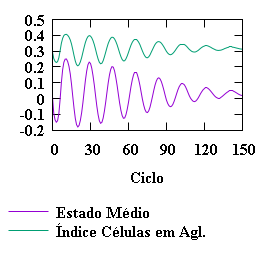
\includegraphics[width=.9\linewidth]{dataL2000Q100CellInClusterAvgStateVsCycle.png}
    \caption{Demonstração da correlação entre o índice de células positivas que pertencem a algum aglomerado e o estado médio do sistema. Quando o estado médio fica mais positivo (existem mais células positivas), o índice de células positivas em aglomerados aumenta proporcionalmente. Analogamente, se o estado médio diminui, o índice de células positivas em aglomerados também diminui.}
    \label{fig:dataL2000Q100CellInClusterAvgStateVsCycle}
\end{figure}
Isso demonstra que esses dois valores estão correlacionados, implicando que as células tendem a estarem aglomeradas. 

Quanto à relação entre o número de aglomerados em função do estado médio, foi constatado que estes tendem a estar relacionados linearmente como na Figura \ref{fig:dataL1750Q100ClustersVsAvgState}. 
\begin{figure}[h]
    \centering
    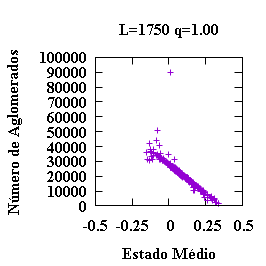
\includegraphics[width=.9\linewidth]{dataL1750Q100ClustersVsAvgState.png}
    \caption{Exemplo da tendência de o número de aglomerados tender a ser linearmente dependente ao estado médio. Este gráfico contém 300 pontos de dados obtidos numa simulação com ajuste máximo de limiar igual a $1.00$ e largura de matriz igual a $1750$. Esse padrão foi observado em todas as outras medições realizadas.}
    \label{fig:dataL1750Q100ClustersVsAvgState}
\end{figure}
Uma análise dos coeficientes angulares das retas que melhor aproximam esses dados (através do Método dos Mínimos Quadrados) para várias larguras de matrizes e vários valores de ajuste máximo de limiar revelou que os gráficos desses coeficientes angulares em função de $q$ apresentam um ``vale'' semelhante ao do potencial de Lennard-Jones, como exibido na Figura \ref{fig:DadosSlopeL1000}.
\begin{figure}
    \centering
    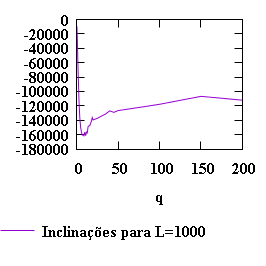
\includegraphics[width=.9\linewidth]{DadosSlopeL1000.png}
    \caption{Exemplo da curva  em função do ajuste máximo de limiar $q$ encontrada para a maioria dos gráficos das inclinações do número de aglomerados \textit{versus} estado médio. Inicialmente foi conjecturada uma semelhança como potencial de Lennard-Jones.}
    \label{fig:DadosSlopeL1000}
\end{figure}
A presença desse ``poço'' em todas as simulações realizadas incentivou a definição da afinidade em função do ajuste máximo de limiar.

\textbf{Definição:} No InCA, seja $I_{q,L}$ a inclinação da reta que melhor aproxima os dados obtidos em uma simulação com ajuste máximo de limiar igual a $q$ e largura de matriz $L$. Seja $Imin_L$ a menor inclinação para um dado $L$. Definimos a \textit{afinidade em função de $q$ e $L$} como sendo $A_{q,L}=-I_{q,L}/Imin_L$.

Contudo, ao analisar a afinidade para várias larguras $L$ diferentes, foi verificado que a Afinidade independe da largura da matriz, como está exibido na Figura \ref{fig:afinidadesQ0a200L750a2000}.
\begin{figure}
    \centering
    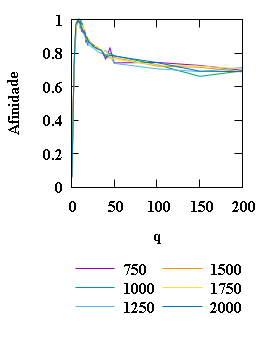
\includegraphics[width=.9\linewidth]{afinidadesQ0a200L750a2000.png}
    \caption{Demonstração da independência da afinidade em relação à largura $L$ da matriz utilizada nas simulações. A sobreposição das seis curvas é aproximadamente absoluta até $q\approx 30$, divergindo levemente entre $q\approx 50$ e $q\approx 200$ devido à natureza estocástica da simulação.}
    \label{fig:afinidadesQ0a200L750a2000}
\end{figure}
Esse fato, corroborado pelo mapa da Figura \ref{fig:afinidadesHeatmap},
incentiva a seguinte definição:

\textbf{Definição:} A \textit{afinidade em função de $q$} é dada pelo valor médio da \textit{afinidade em função de $q$ e $L$} através de várias medições para vários valores de $L$.

Com base nessa definição, foi encontrado o gráfico da afinidade através das simulações realizadas. Esse gráfico está exibido na Figura \ref{fig:afinidadeMedia}.

Também foram buscados padrões de caos e atratores na dinâmica não-linear das simulações realizadas, sendo encontrados vários gráficos com comportamentos interessantes, como o da Figura \ref{fig:dataL1000Q75ClustersVsAvgThres}. Contudo, ainda não foi verificado se existe caos nesses sistemas.

Por fim foram feitas simulações considerando matrizes em três dimensões, nas quais foi possível constatar comportamentos análogos aos observados no caso de duas dimensões, como a relação entre estado médio e limiar médio em função do ciclo de simulação, além da linearidade do número de aglomerados em função do estado médio. Trabalhos nessas simulações foram descontinuados devido a incertezas sobre a precisão do código utilizado.

\section*{Conclusão}

Com os trabalhos desenvolvidos neste semestre foi possível desenvolver habilidades de análise e reprodução de autômatos celulares (em especial o \textit{Inhomogenous Cellular Automata} de Stauffer). A grande surpresa do estudo aconteceu nos recorrentes padrões lineares no caso dos gráficos do número de aglomerados em função do estado médio, sendo ainda mais surpreendente a independência da afinidade em relação à largura da matriz utilizada. A existência de discos como atratores de vários dos gráficos de número número de aglomeros em função do limiar médio também foi inesperada. Dos estudos relacionados à simulações em três dimensões, foi fortalecida a necessidade de códigos de programação bem organizados, a fim de evitar incertezas sobre a validade dos resultados.

Os próximos passos incluem estudar o motivo da existência do máximo no gráfico da afinidade média (Figura \ref{fig:afinidadeMedia}), possivelmente relacionando-o ao potencial de Lennard-Jones, analisar os atratores nos gráficos do número de aglomerados em função do limiar médio utilizando teoria de dinâmica não-linear e caos, e explorar autômatos não lineares em dimensões maiores do que 2.

\begin{figure}
    \centering
    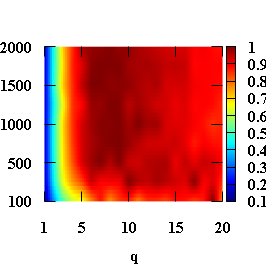
\includegraphics[width=.9\linewidth]{afinidadesHeatmap.png}
    \caption{Gráfico em três dimensões da afinidade (de $0$ a $1$ em cores de azul à vermelho de acordo com legenda na lateral direita) em função do valor máximo de ajuste de limiar $q$, para cada largura $L$ de matriz entre $100$ e $2000$. É perceptível que, para a maioria das linhas (valores fixos de L), o padrão de cores é semelhante. Esse padrão é diferente para valores próximos de $L=100$, nos quais existe grande instabilidade na simulação, provavelmente devido aos efeitos das células nas bordas, pois estas têm menos vizinhos que as demais células.}
    \label{fig:afinidadesHeatmap}
\end{figure}

\begin{figure}
    \centering
    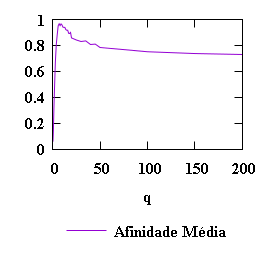
\includegraphics[width=.9\linewidth]{afinidadeMedia.png}
    \caption{Resultado da computação da afinidade média com base nas 288 simulações realizadas. A presença de um máximo em $q\approx 8$ levantou conjecturas que ainda hão de ser verificadas.}
    \label{fig:afinidadeMedia}
\end{figure}

\begin{figure}
    \centering
    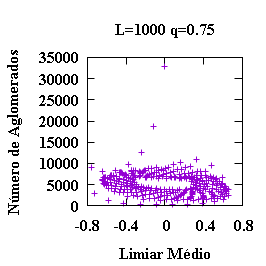
\includegraphics[width=.9\linewidth]{dataL1000Q75ClustersVsAvgThres.png}
    \caption{Padrão de atrator em formato de disco encontrado no gráfico do número de aglomerados em função do limiar médio para várias larguras $L$ e valores de ajuste máximo de limiar $q$. O ponto inicial está em aproximadamente $(0,32500)$.}
    \label{fig:dataL1000Q75ClustersVsAvgThres}
\end{figure}

\begin{thebibliography}{9}
	
	\bibitem{britannica1}
	BRITANNICA, Encyclopaedia.
	\textbf{``Automaton''}, 
	\textit{Acessado em 14 de Dezembro de 2018}.
	\url{https://www.britannica.com/technology/automaton}
	
	\bibitem{britannica2}
	BRITANNICA, Encyclopaedia.
	\textbf{``Automata theory''}, 
	\textit{Acessado em 14 de Dezembro de 2018}.
	\url{https://www.britannica.com/topic/automata-theory}
	
	\bibitem{britannica3}
	BRITANNICA, Encyclopaedia.
	\textbf{``Cellular automata''}, 
	\textit{Acessado em 14 de Dezembro de 2018}.
	\url{https://www.britannica.com/science/cellular-automata}
	
	\bibitem{king}
	KING, K. N.
	\textbf{``C Programming: a modern approach, second edition''}, 
	\textit{ W. W. Norton \& Company, Abril de 2008}.
	
	\bibitem{klaus}
	KRAMER, Klaus.
	\textbf{``Dinâmica de padrões em autômatos celulares com inércia''}, 
	\textit{ UFPR, Curitiba-PR, 2014}.
	
	\bibitem{lazzari}
	LAZZARI, Rodrigo de.
	\textbf{``Estudo de um autômato celular para modelar ciclos de expansão e constração (\textit{boom} e \textit{burst})''}, 
	\textit{ UFPR, Curitiba-PR, 2018}.
	
	\bibitem{netlogo}
	\textbf{``NetLogo ver. 6.0.4''}, 
	\textit{Uri Wilensky, 2016}.
	\url{ccl.northwestern.edu/netlogo/}

	\bibitem{stauffer}
	STAUFFER, Dietrich; WEISBUCH, Gérard.
	\textbf{``Adjustment and social choice''}, 
	\textit{ Elsevier, Physica A 323 (2003) 651-662}.
	
	\bibitem{wolfram}
	WOLFRAM, Stephen.
	\textbf{``A new kind of Science, Online''}, 
	\textit{Stephen Wolfram, 2018}. URL: \url{www.wolframscience.com/nks/}
	
\end{thebibliography}

\end{document}
